\chapter{Estymacja w modelu Coxa metodą stochastycznego spadku gradientu}\label{rozdz4}

Poniższy rozdział przedstawia implementację oraz zastosowanie metody stochastycznego spadku gradientu do estymacji współczynników w modelu proporcjonalnych hazardów Coxa. Jest to główny cel pracy. Przedstawione rozważania odnośnie omawianego podejścia są nowatorskie, dlatego nie mogą być poparte literaturą naukową.

W czasie powstawania pracy nawiązano jedynie krótką wymianę informacji z pracownikami \textit{Harvard Laboratory for Applied Statistical Methodology \& Data Science}, dzięki której dowiedziano się, że podjęte zostały kroki w kierunku stworzenia podwalin pod teorię do omawianego zagadnienia, jednak ewentualne publikacje nie zostały jeszcze dokończone. Przedsmak zaimplementowanego podobnego algorytmu przez pracowników wyżej wymienionego laboratorium można znaleźć w \cite{sgdpkg}.

W procesie estymacji współczynników w omawianym modelu wykorzystano pochodne cząstkowe częściowej funkcji log-wiarogodności (\ref{score})
\begin{equation*}
U_k(\beta)=\dfrac{\partial{}_{p}\ell_k(\beta)}{\partial\beta_k}=\sum\limits_{i=1}^{K}\left(X_{ik}-\dfrac{\sum\limits_{l\in \mathscr{R}(t_i)}^{} X_{lk} e^{X_l'\beta}}{\sum\limits_{l\in \mathscr{R}(t_i)}^{} e^{X_l'\beta}}\right)=\sum\limits_{i=1}^{n}Y_i\left(X_{ik}-\dfrac{\sum\limits_{l\in \mathscr{R}(t_i)}^{} X_{lk} e^{X_l'\beta}}{\sum\limits_{l\in \mathscr{R}(t_i)}^{} e^{X_l'\beta}}\right)=\sum\limits_{i=1}^{n}U_{k,i}(\beta),
\end{equation*}
($Y_i = 1$, gdy obserwacja nie była cenzurowana i $Y_i = 0$, gdy obserwacja była cenzurowana; $K$ to liczba zdarzeń; $n$ to liczba obserwacji) oraz wzór (\ref{sgdrownanie}), którego wersja z adekwatnymi oznaczeniami do powyższej funkcji wygląda następująco
\begin{equation}\label{opta}
\beta_{k,j+1} = \beta_{k,j} - \alpha_{j}U_{k,i}(\beta_{k,j}),
\end{equation}
gdzie $j$ oznacza krok algorytmu, $i$ iteruje składniki $U_{k}$, $\alpha_j$ to długość $j$-tego kroku algorytmu, zaś $U_{k}$ to $k$-ta pochodna cząstkowa gradientu $U$ oraz $\beta_{k,j}$ to (dla $j$-tego kroku) $k$-ta współrzędna estymowanego wektora współczynników $\beta$ o rozmiarze $p$, czyli $k=1,\dots,p$. 

Własna implementacja algorytmu w języku $\mathcal{R}$ znajduje się w podrozdziale (\ref{implemento}).

\section{Założenia i obserwacje}\label{zalozenia}

Skupiając się na informatycznym aspekcie algorytmu można stwierdzić, że idea stochastycznego spadku gradientu polega na losowaniu składnika optymalizowanej funkcji. Jednak ze statystycznego punktu widzenia, metoda stochastycznego spadku gradientu opiera się o losowanie indeksu obserwacji ze zbioru, z którego uczony jest algorytm, zanim postanowi się w jakikolwiek sposób przedstawić konkretną funkcję wiarogodności. Zatem w celu estymacji, w oparciu o stochastyczny spadek gradientu w modelu Coxa, konstruując metodę należy najpierw losować obserwacje, a następnie dopiero wyznaczać formę optymalizowanej funkcji częściowej log-wiarogodności. 

Dla wielu modeli opierających się o funkcje wiarogodności te dwa punkty widzenia są równoważne, jednak nie w przypadku modelu Coxa nie, gdzie niektóre składniki w funkcji log-wiarogodności są zależne od poprzednich obserwacji. W przypadku modelu ADALINE sformułowanego jak w \cite{ADALINE2}, opartego na minimalizowaniu funkcji kosztu w~postaci błędu najmniejszych kwadratów, w \cite{bott2} podano postać funkcji straty oraz równanie algorytmu stochastycznego spadku gradientu jak poniżej
$$Q(w) = \frac{1}{2}(y-w'\varPhi(x))^2, \ \ \ \varPhi(x) \in \mathbb{R}^d, y \in \{-1,1\},$$ 
$$w \leftarrow w + \alpha_k(y_k-w'\varPhi(x_t))\varPhi(x_t),$$
przy których widać, że w kolejnych krokach algorytmu $t$ wystarczy tylko jedna obserwacja $z_t=(x_t,y_t)$ aby poprawić oszacowanie parametru $w$.

W modelu proporcjonalnych hazardów Coxa jest to bardziej skomplikowane. Mając z~góry zadaną funkcję hazardu, częściowa funkcja wiarogodności odpowiada prawdopodobieństwu tego, że obserwowane zdarzenia zdarzyłyby się dokładnie w tej kolejności w jakiej się pojawiły. To~prawdopodobieństwo zależy od wszystkich obserwacji w zbiorze. Niemożliwe jest wyliczenie tego poprzez obliczenie wartości funkcji częściowej wiarogodności oddzielnie dla obserwacji o~numerach od 1 do 5 i oddzielnie dla obserwacji od numerach 6 do 10, a~następnie przemnożeniu wyników przez siebie. Z tej przyczyny niemożliwe jest losowanie czynników optymalizowanej funkcji przy użyciu metody stochastycznego spadku gradientu do estymacji współczynników w tym modelu. Alternatywnym podejściem do tego problemu mogłoby być pamiętanie wartości licznika i mianownika w składnikach częściowej funkcji log-wiarogodności, dla wszystkich zaobserwowanych czasów zdarzeń i poprawianie odpowiednich składników, z~wykorzystaniem świeżych obserwacji. Taki zabieg jest pamięciowo oszczędniejszy niż wykorzystywanie całego zbioru danych. \textbf{Innym rozwiązaniem jest losowanie podzbioru obserwacji, a następnie konstruowanie funkcji wiarogodności dla zaobserwowanego zredukowanego zbioru. Właśnie ta metoda zostanie opisana w~dalszej części pracy.} Taki sposób wprowadzania obserwacji do estymacji można wykorzystać w sytuacjach, gdy ma się do czynienia z nieskończonym napływem nowych obserwacji, a~potrzebne jest oszacowanie estymowanych parametrów modelu $\beta_k, k=1,\dots,p$ dla obecnie zaobserwowanych i~wykorzystanych obserwacji. Proces ten ma dwie zalety: nie dość, że dla nowych obserwacji model jest w stanie na bazie obecnych oszacowań parametrów dokonać predykcji proporcji hazardów, to dodatkowo po każdej porcji obserwacji aktualizuje parametry modelu.

Ponieważ
omawiane algorytmy rozwiązują problem minimalizacji badanej funkcji, zaś
celem estymacji w modelu Coxa jest znalezienie parametrów modelu
maksymalizujących funkcję częściowej log-wiarogodności, zatem wzięcie do
minimalizacji funkcji z przeciwnym znakiem doprowadzi do wykorzystania
metod znajdujących minimum do znalezienia maksimum. 

Zakładając,~że w~\(j\)-tym kroku
algorytmu i przy \(k\)-tej pochodnej cząstkowej dysponuje się zaobserwowanym podzbiorem
\(\mathcal{B}\), częściową funkcję wiarogodności dla zaobserwowanego podzbioru obserwacji \(\mathcal{B}\) wykorzystywaną do minimalizacji można zapisać następująco
\begin{equation}
-U^\mathcal{B}_k(\beta_{.,j})=-\sum\limits_{i \in \mathcal{B}_\text{ind}}^{}U^\mathcal{B}_{k,i}(\beta_{.,j})=-\sum\limits_{i \in \mathcal{B}_\text{ind}}^{}Y_i\left(X_{ik}-\dfrac{\sum\limits_{l\in \mathscr{R}_\mathcal{B}(t_i)}^{} X_{lk} e^{X_l'\beta_{.,j}}}{\sum\limits_{l\in \mathscr{R}_\mathcal{B}(t_i)}^{} e^{X_l'\beta_{.,j}}}\right),
\end{equation}
gdzie indeksy obserwacji należące do \(\mathcal{B}\) definiuje się jako
\(\mathcal{B}_{\text{ind}} = \{i: X_i \in \mathcal{B} \}\), zaś
\(\mathscr{R}_\mathcal{B}(t_i)\) to zbiór ryzyka dla zbioru
\(\mathcal{B}\) w czasie \(t_i\), a $\beta_{.,j}$ to wektor współczynników w $j$-tym kroku.

Postać powyższej funkcji nasuwa pewne obserwacje. W danym kroku algorytmu, obecnie wykorzystywany zaobserwowany podzbiór obserwacji \(\mathcal{B}\)
\begin{itemize}
\item \textit{nie powinien składać się jedynie z obserwacji cenzurowanych} \newline \ \newline Dla podzbioru zawierającego jedynie takie obserwacje wartość pochodnej cząstkowej funkcji log-wiarogodności jest równa zero, ze względu na czynniki $Y_i$, które dla obserwacji cenzurowanych są równe zero. Zerowa wartość pochodnej cząstkowej funkcji log-wiarogodności doprowadzi do niezmienienia się optymalizowanych parametrów we wzorze (\ref{opta}), a co za tym idzie, doprowadzi do przerwania optymalizacji.
\item \textit{nie powinien składać się jedynie z jednej obserwacji} \newline \ \newline  
W takim przypadku wartość pochodnej cząstkowej funkcji log-wiarogodności jest również równa zero, bez względu na to czy obserwacja była cenzurowana czy nie, gdyż 
$$-U_{k}^{\mathcal{B}}(\beta{.,j})=-Y_m\left(X_{mk}-\dfrac{ X_{mk} e^{X_m'\beta_{.,j}}}{ e^{X_m'\beta_{.,j}}}\right) = -Y_m\left(X_{mk}-X_{mk}\right) = -Y_m \cdot 0 = 0,$$
dla dowolnego $m$ oznaczającego indeks jedynej obserwacji w $\mathcal{B}$, czyli $\mathcal{B}_{\text{ind}}=\{m\}$. 
\item \textit{nie powinien zawierać tylko jednej obserwacji niecenzurowanej w zbiorze, która dodatkowo ma największy czas bycia pod obserwacją} \newline \ \newline 
W tej sytuacji jedyny niezerowy czynnik w całej pochodnej cząstkowej funkcji log-wiarogodności zajdzie tylko dla obserwacji niecenzurowanej, dla której zbiór ryzyka będzie zawierał tylko ją samą, co da ostatecznie zerową wartość pochodnej cząstkowej optymalizowanej funkcji log-wiarogodności i doprowadzi do przerwania optymalizacji.
\end{itemize}

Dodatkowo nie dochodzi do wykorzystania obserwacji cenzurowanych, gdy:
\begin{itemize}
\item \textit{zaobserwowany zbiór zawiera obserwacje cenzurowane, które wszystkie mają czasy obserwacji krótsze niż najmniejszy czas obserwacji dla obserwacji niecenzurowanej} \newline \ \newline 
Obserwacje cenzurowane niosą ze sobą mniej informacji, jednak teoria analizy przeżycia stara się je maksymalnie wykorzystać. Stąd uwzględnia się ich udział w~zbiorze ryzyka przy estymacji fragmentów funkcji log-wiarogodności dla obserwacji niecenzurowanych. W sytuacji, gdy wszystkie obserwacje cenzurowane mają czas obserwacji krótszy niż najmniejszy czas obserwacji dla obserwacji niecenzurowanej w~podzbiorze, nie dochodzi do wykorzystania obserwacji cenzurowanych w~jakikolwiek sposób przy estymacji współczynników w danym kroku algorytmu.
\end{itemize}

Mając na względzie te uwagi, w sytuacji gdy zaobserwuje się podzbiór, który spełnia jeden z wyżej wymienionych warunków, zamiast wykorzystywać ten zbiór do estymacji można go dołączyć do kolejnego podzbioru, który ma być zaobserwowany.

\newpage
\section{Implementacja}\label{implemento}

Omówiona w tym rozdziale metoda estymacji metodą stochastycznego spadku gradientu w~modelu proporcjonalnych hazardów Coxa została zaimplementowana w języku $\mathcal{R}$ i~jest dostępna w specjalnie przygotowanym pakiecie o nazwie \texttt{coxphSGD()}, który można jednocześnie pobrać z internetu i zainstalować poleceniem
\begin{Shaded}
\begin{Highlighting}[]
\NormalTok{devtools::}\KeywordTok{install_github}\NormalTok{(}\StringTok{"MarcinKosinski/coxphSGD"}\NormalTok{)}
\end{Highlighting}
\end{Shaded}

Dokumentacja wraz z opisem argumentów w języku angielskim funkcji \texttt{coxphSGD()}, która estymuje współczynniki w modelu
proporcjonalnych hazardów Coxa metodą stochastycznego spadku gradientu, dostępna jest w Dodatku \ref{docCoxSGD}.
Starano się zachować jednorodność kolejności i nazewnictwa parametrów z funkcją \texttt{coxph()} z pakietu \texttt{survival} \citep{ther, survival}.

Implementacja algorytmu estymacji w modelu Coxa metodą stochastycznego spadku gradientu opiera się na poniższym pseudo-kodzie i zakłada, że kolejne podzbiory \(\mathcal{B}\) dostarczane są jako kolejne elementy listy.
\subsubsection{Estymacja~w~modelu~Coxa~metodą~stochastycznego~spadku~gradientu}


\begin{Shaded}
\begin{Highlighting}[]
                    \CommentTok{# wstępna inicjalizacja parametrów}
\NormalTok{eps =}\StringTok{ }\FloatTok{1e-5}                               \CommentTok{# warunek stopu.}

\NormalTok{n =}\StringTok{ }\KeywordTok{length}\NormalTok{(data)                         }\CommentTok{# data jest listą ramek danych.}

\NormalTok{diff =}\StringTok{ }\NormalTok{eps +}\StringTok{ }\DecValTok{1}                           \CommentTok{# różnice w oszacowaniach parametrów}
                                         \CommentTok{# między kolejnymi krokami.}

\NormalTok{learningRates =}\StringTok{ }\NormalTok{function(x) }\DecValTok{1}\NormalTok{/x          }\CommentTok{# długości kroku algorytmu.}

\NormalTok{beta_old =}\StringTok{ }\KeywordTok{numeric}\NormalTok{(}\DecValTok{0}\NormalTok{, }\DataTypeTok{length =} \NormalTok{k)        }\CommentTok{# punkt startowy dlugosci k,}
                                         \CommentTok{# gdzie k to liczba zmiennych}
                                         \CommentTok{# objaśniających w modelu.}

\NormalTok{max.iter =}\StringTok{ }\DecValTok{500}                           \CommentTok{# maksymalna liczba kroków.}

                              \CommentTok{# estymacja}
\NormalTok{i =}\StringTok{ }\DecValTok{1}                                    \CommentTok{# iterator kroku algorytmu.}
\NormalTok{while(i <=}\StringTok{ }\NormalTok{max.iter \&}\StringTok{ }\NormalTok{diff <}\StringTok{ }\NormalTok{eps) do     }
  \NormalTok{iter =}\StringTok{ }\KeywordTok{ifelse}\NormalTok{(i mod n ==}\StringTok{ }\DecValTok{0}\NormalTok{, n, i mod n)}\CommentTok{# wybierz kolejny podzbiór batch.}
  \NormalTok{batch =}\StringTok{ }\NormalTok{data[[iter]] }
  \NormalTok{beta_new =}\StringTok{ }\NormalTok{beta_old -}\StringTok{ }\KeywordTok{learningRates}\NormalTok{(i) *}\StringTok{ }\KeywordTok{U_Batch}\NormalTok{(batch) }
                                         \CommentTok{# U_Batch to gradient częściowej funkcji}
                                         \CommentTok{# log-wiarogdności dla zaobserwowanego}
                                         \CommentTok{# zbioru `batch`.}
  \NormalTok{diff =}\StringTok{ }\KeywordTok{euclidean_dist}\NormalTok{(beta_new, beta_old) }\CommentTok{# odległość euklidesowa}
  \NormalTok{beta_old =}\StringTok{ }\NormalTok{beta_new }
  \NormalTok{i =}\StringTok{ }\NormalTok{i +}\StringTok{ }\DecValTok{1}
\NormalTok{end while}
\NormalTok{return beta_new}
\end{Highlighting}
\end{Shaded}

\textbf{Docelowa implementacja w języku $\mathcal{R}$ znajduje się poniżej.} \newline \ \newline

\begin{Shaded}
\begin{Highlighting}[]
\NormalTok{coxphSGD <-}\StringTok{ }\NormalTok{function(formula, data, }\DataTypeTok{learningRates =} \NormalTok{function(x)\{}\DecValTok{1}\NormalTok{/x\},}
                    \DataTypeTok{beta_0 =} \DecValTok{0}\NormalTok{, }\DataTypeTok{epsilon =} \FloatTok{1e-5}\NormalTok{, }\DataTypeTok{max.iter =} \DecValTok{500} \NormalTok{) \{}
  \CommentTok{# check arguments}
  \KeywordTok{checkArguments}\NormalTok{(formula, data, learningRates,}
                  \NormalTok{beta_0, epsilon) ->}\StringTok{ }\NormalTok{beta_start }
  \NormalTok{n <-}\StringTok{ }\KeywordTok{length}\NormalTok{(data)}
  \NormalTok{diff <-}\StringTok{ }\NormalTok{epsilon +}\StringTok{ }\DecValTok{1}
  \NormalTok{i <-}\StringTok{ }\DecValTok{1}
  \NormalTok{beta_new <-}\StringTok{ }\KeywordTok{list}\NormalTok{()     }\CommentTok{# steps are saved in a list so that they can}
  \NormalTok{beta_old <-}\StringTok{ }\NormalTok{beta_start }\CommentTok{# be traced in the future}
  \CommentTok{# estimate}
  \NormalTok{while(i <=}\StringTok{ }\NormalTok{max.iter &}\StringTok{ }\NormalTok{diff >}\StringTok{ }\NormalTok{epsilon) \{}
    \NormalTok{beta_new[[i]] <-}\StringTok{ }\KeywordTok{coxphSGD_batch}\NormalTok{(}\DataTypeTok{formula =} \NormalTok{formula, }\DataTypeTok{beta =} \NormalTok{beta_old,}
        \DataTypeTok{learningRate =} \KeywordTok{learningRates}\NormalTok{(i), }\DataTypeTok{data =} \NormalTok{data[[}\KeywordTok{ifelse}\NormalTok{(i%%n==}\DecValTok{0}\NormalTok{,n,i%%n)]]) %>%}
\StringTok{      }\NormalTok{unlist}
    \NormalTok{diff <-}\StringTok{ }\KeywordTok{sqrt}\NormalTok{(}\KeywordTok{sum}\NormalTok{((beta_new[[i]] -}\StringTok{ }\NormalTok{beta_old)^}\DecValTok{2}\NormalTok{))}
    \NormalTok{beta_old <-}\StringTok{ }\NormalTok{beta_new[[i]]}
    \NormalTok{i <-}\StringTok{ }\NormalTok{i +}\StringTok{ }\DecValTok{1}
    \KeywordTok{cat}\NormalTok{(}\StringTok{"}\CharTok{\textbackslash{}r}\StringTok{ iteration: "}\NormalTok{, i, }\StringTok{"}\CharTok{\textbackslash{}r}\StringTok{"}\NormalTok{)}
  \NormalTok{\}  }
  \CommentTok{# return results}
  \KeywordTok{list}\NormalTok{(}\DataTypeTok{Call =} \KeywordTok{match.call}\NormalTok{(), }\DataTypeTok{epsilon =} \NormalTok{epsilon,}
       \DataTypeTok{learningRates =} \NormalTok{learningRates, }\DataTypeTok{steps =} \NormalTok{i,}
       \DataTypeTok{coefficients =} \KeywordTok{c}\NormalTok{(}\KeywordTok{list}\NormalTok{(beta_start), beta_new))}
\NormalTok{\}}

\NormalTok{coxphSGD_batch <-}\StringTok{ }\NormalTok{function(formula, data, learningRate, beta)\{}
  \CommentTok{# collect times, status, variables and reorder samples }
  \CommentTok{# to make the algorithm more clear to read and track}
  \NormalTok{batchData <-}\StringTok{ }\KeywordTok{prepareBatch}\NormalTok{(}\DataTypeTok{formula =} \NormalTok{formula, }\DataTypeTok{data =} \NormalTok{data)}
  \CommentTok{# calculate the log-likelihood for this batch sample}
  \NormalTok{batchData <-}\StringTok{ }\NormalTok{batchData %>%}\StringTok{ }\KeywordTok{arrange}\NormalTok{(-times)}
  \CommentTok{# scores occure in nominator and denominator}
  \NormalTok{scores <-}\StringTok{ }\KeywordTok{apply}\NormalTok{(batchData[, -}\KeywordTok{c}\NormalTok{(}\DecValTok{1}\NormalTok{, }\DecValTok{2}\NormalTok{)], }\DecValTok{1}\NormalTok{, }
                  \NormalTok{function(element) }\KeywordTok{exp}\NormalTok{(element %*%}\StringTok{ }\NormalTok{beta) )}
  \NormalTok{nominator <-}\StringTok{ }\KeywordTok{apply}\NormalTok{(batchData[, -}\KeywordTok{c}\NormalTok{(}\DecValTok{1}\NormalTok{, }\DecValTok{2}\NormalTok{)], }\DecValTok{2}\NormalTok{,}
                         \NormalTok{function(element) }\KeywordTok{cumsum}\NormalTok{(scores*element) )}
  \NormalTok{denominator <-}\StringTok{ }\KeywordTok{cumsum}\NormalTok{(scores)}
  \CommentTok{# sum over non-censored observations}
  \NormalTok{partial_sum <-}\StringTok{ }\NormalTok{(batchData[, -}\KeywordTok{c}\NormalTok{(}\DecValTok{1}\NormalTok{, }\DecValTok{2}\NormalTok{)] -}\StringTok{ }\NormalTok{nominator/denominator)*batchData[, }\StringTok{"event"}\NormalTok{]}
  \CommentTok{# each column indicates one explanatory variable  }
  \NormalTok{U_batch <-}\StringTok{ }\NormalTok{partial_sum %>%}\StringTok{ }\KeywordTok{colSums}\NormalTok{()}
  \KeywordTok{return}\NormalTok{(beta +}\StringTok{ }\NormalTok{learningRate *}\StringTok{ }\NormalTok{U_batch)}
\NormalTok{\}}
\end{Highlighting}
\end{Shaded}
\newpage
\section{Symulacje estymacji w modelu Coxa}

Dzięki przygotowanej w rozdziale \ref{symWei} funkcji \texttt{dataCox()} możliwe będzie symulacyjne zbadanie zachowania się współczynników w modelu Coxa w trakcie estymacji metodą stochastycznego spadku gradientu, której algorytm został zaimplementowany w rozdziale \ref{implemento}. Poniższe wywołanie zwraca ramkę danych o 10 tysiącach wierszy, wraz ze sztucznie wygenerowanymi czasami z rozkładu Weibulla o parametrach $\lambda =3$ oraz $\rho =2$. Czasy cenzurowania generowane są z rozkładu wykładniczego o parametrze $0.2$, a ostateczne czasy bycia pod obserwacją odpowiadają współczynnikom modelu $\beta = (1,3)$. Porównując czas życia oraz czas cenzurowania wylosowany dla obserwacji, w rezultacie otrzymać można czasy przeżycia oraz status zdarzenia bądź cenzurowania. 
\begin{Shaded}
\begin{Highlighting}[]
\NormalTok{x <-}\StringTok{ }\KeywordTok{matrix}\NormalTok{(}\KeywordTok{sample}\NormalTok{(}\DecValTok{0}\NormalTok{:}\DecValTok{1}\NormalTok{, }\DataTypeTok{size =} \DecValTok{20000}\NormalTok{, }\DataTypeTok{replace =} \OtherTok{TRUE}\NormalTok{), }\DataTypeTok{ncol =} \DecValTok{2}\NormalTok{)}
\NormalTok{dCox <-}\StringTok{ }\KeywordTok{dataCox}\NormalTok{(}\DecValTok{10}\NormalTok{^}\DecValTok{4}\NormalTok{, }\DataTypeTok{lambda =} \DecValTok{3}\NormalTok{, }\DataTypeTok{rho =} \DecValTok{2}\NormalTok{, x, }\DataTypeTok{beta =} \KeywordTok{c}\NormalTok{(}\DecValTok{1}\NormalTok{,}\DecValTok{3}\NormalTok{), }\DataTypeTok{censRate =} \DecValTok{0.2}\NormalTok{) }
\end{Highlighting}
\end{Shaded}
Funkcja \texttt{simulateCoxSGD()} opisana w Dodatku \ref{coxKody123} pięciokrotnie dzieli wygenerowany zbiór danych odpowiednio na 30, 60, 90, 120 i 200 podzbiorów losowych długości ustawiając obserwacje w losowej kolejności, a następnie wykorzystuje funkcję \texttt{coxphSGD()} do wyznaczenia wartości współczynników w kolejnych krokach estymacji funkcji log-wiarogodności w modelu Coxa przy pomocy metody stochastycznego spadku gradientu. Dzięki tak otrzymanym współczynnikom modelu w kolejnych krokach algorytmu przy różnych podziałów zbiorów, możliwe było graficzne przedstawienie trajektorii zbieżności algorytmu w zależności od punktu startowego, warunku stopu oraz wartości ciągu odpowiadającego długościom kroków. 

Implementacja umożliwia ponowne wykorzystanie wszystkich zaobserwowanych podzbiorów danych w kolejnych krokach algorytmu, jeżeli nie pozostały już do wykorzystania żadne nowe podzbiory, zaś zbieżność algorytmu, poza warunkiem stopu, zależna jest także od maksymalnej liczby iteracji, która jest większa od liczby zaobserwowanych podzbiorów. Jednorazowe wykorzystanie wszystkich obserwacji w trakcie procesu optymalizacji nazywane jest \textit{epoką}. 

Przykładowe wywołanie funkcji \texttt{simulateCoxSGD()} znajduje się poniżej

\begin{Shaded}
\begin{Highlighting}[]
\KeywordTok{simulateCoxSGD}\NormalTok{(dCox, }\DataTypeTok{learningRates =} \NormalTok{function(x)\{}\DecValTok{1}\NormalTok{/(}\DecValTok{100}\NormalTok{*}\KeywordTok{sqrt}\NormalTok{(x))\},}
               \DataTypeTok{max.iter =} \DecValTok{10}\NormalTok{, }\DataTypeTok{epsilon =} \FloatTok{1e-5}\NormalTok{, }\DataTypeTok{beta_0 =} \KeywordTok{c}\NormalTok{(}\DecValTok{2}\NormalTok{,}\DecValTok{2}\NormalTok{))}
\end{Highlighting}
\end{Shaded}
gdzie w tym wypadku parametr \texttt{max.iter} odpowiada za liczbę epok do wykorzystania, \texttt{learningRates} to funkcja odpowiedzialna za wyznaczenie długości kolejnych kroków algorytmu, \texttt{dCox} to dane do analizy przygotowane w postaci jaką zwraca funkcja \texttt{dataCox()}, \texttt{epsilon} to warunek stopu, zaś \texttt{beta\_0} to punkt startowy algorytmu.

Na Rysunkach \ref{rysCox} - \ref{rysCox4} przedstawiono symulacje zbieżności procesu optymalizacji częściowej funkcji log-wiarogodności w modelu Coxa proporcjonalnych hazardów, konstruowanej jedynie dla zaobserwowanego w danym kroku podzbioru obserwacji, z wykorzystaniem algorytmu stochastycznego spadku gradientu. Trajektorie zbieżności zależne są od ustawionego punktu startowego, warunku stopu oraz wartości ciągu odpowiadającego długościom kroków w algorytmie. Dodatkowo elipsami przedstawiono warstwice częściowej funkcji log-wiarogodności wyliczone mając wszystkie zaobserwowane podzbiory połączone w jeden. Trójkątem zaznaczono punkt startowy algorytmu, kwadratem teoretyczne maksimum, zaś gwiazdką współczynniki uzyskane za pomocą funkcji \texttt{coxph()}, która znajduje rozwiązania przy pomocy algorytmu spadku gradientu rzędu II (Raphsona-Newtona).

\newpage
\subsubsection{Podsumowanie symulacji w modelu proporcjonalnych hazardów Coxa}

W trakcie symulacji badano jak podział całego zbioru obserwacji na podzbiory wpływa na trajektorie optymalizacji częściowej funkcji log-wiarogodności w modelu Coxa proporcjonalnych hazardów, konstruowanej na bazie zaobserwowanego podzbioru. Badano również wpływ punktu początkowego, warunku stopu, liczby epok oraz konstrukcji ciągu odpowiedzialnego za długości kroków na proces optymalizacji w tym modelu. 

Na Rysunkach \ref{rysCox} - \ref{rysCox4} ukazano trajektorie powstałe przy punktach początkowych
 $$\beta_0 = (0,0), (2,2), (-1,4),$$
 gdzie pod uwagę brano ciągi odpowiadające długościom kroków takie jak 
 $$\alpha_t=\frac{1}{20\sqrt{t}}, \ \ \alpha_t = \frac{1}{50\sqrt{t}}, \ \ \alpha_t = \frac{1}{100\sqrt{t}}.$$ 
 Eksperymentowano z liczbą epok ustalaną na $1,5,10$ oraz sprawdzano jak zachowają się trajektorie z warunkami stopu $\varepsilon=10^{-6}$ lub $\varepsilon=10^{-5}$. Przy ciągach odpowiadających za długości kroków ustalonych na  
 $$\alpha_t=\frac{1}{20t}, \ \ \alpha_t = \frac{1}{50t}, \ \ \alpha_t = \frac{1}{100t}$$
   algorytm nie osiągał zbieżności i zatrzymywał się po maksymalnej liczbie iteracji w losowym punkcie znacznie odległym od optimum.

W każdej z symulacji algorytm zbiegł do punktu, w którym powinno być teoretyczne optimum. W wielu wypadkach już po jednej epoce. Może to oznaczać, że opisana metoda dobrze sprawdza się w sytuacji napływających danych. Należy zaznaczyć, że przy odmiennych sprawdzanych wariantach procesu optymalizacji, za każdym razem metoda zbiegała prostopadle do ukazanych warstwic częściowej funkcji log-wiarogodności konstruowanej na bazie \textbf{całych} danych. Jest to jasny sygnał świadczący za poprawnością wyliczania wartości gradientu częściowej funkcji log-wiarogodności, konstruowanej na bazie zaobserwowanego podzbioru. Co~więcej, stochastyczny spadek gradientu nie wykorzystuje wszystkich obserwacji jednocześnie, przez co trudniej jest mu zbiec do teoretycznego optimum, a jednak w opisanej sytuacji algorytm osiągnął cel, dodatkowo zyskując na szybkości zbieżności i złożoności obliczeniowej. Warta podkreślenia jest stabilność procesu optymalizacji wśród ciągów odpowiadających za długość kroków, które ustawione zostały na mniejsze wartości (Rysunki \ref{rysCox} - \ref{rysCox3}). Ostatecznie należy zwrócić uwagę na fakt, że większa liczba epok i mniejszy warunek stopu powodują jedynie poprawienie optymalizacji dla wariantów, w których cały zbiór obserwacji był podzielony na największą liczbę podzbiorów, a więc każdy krok algorytmu budowany był na najmniej licznych podzbiorach. W pozostałych przypadkach nie poprawia to optymalizacji. Można sądzić, że im liczniejszy zaobserwowany podzbiór tym skuteczniejsza estymacja.

Proces estymacji w modelu proporcjonalnych hazardów Coxa z wykorzystaniem metody stochastycznego spadku gradientu w sytuacji napływających danych jest stabilny i~zbiega w~okolice bliskie teoretycznemu optimum, niekiedy nawet już po jednej epoki. Przy dobrze dobranych parametrach optymalizacji, proces może być z powodzeniem wykorzystywany do znajdowania współczynników modelu. Kluczowym momentem mającym wpływ na powodzenie optymalizacji jest wybór ciągu odpowiedzialnego za dobór długości kroków w~algorytmie, więc zaleca się symulacje badające odmienne ciągi oraz wybranie tego ciągu, który w~większości przypadków daje stabilne, jednorodne współczynniki, maksymalizujące częściową funkcję wiarogodności konstruowaną na bazie oddzielnego zbioru testowego.

\newpage

\begin{figure}[hbt!]
  %\vspace{-10pt}
  \begin{center}
   \begin{subfigure}[h!]{0.9\textwidth}
      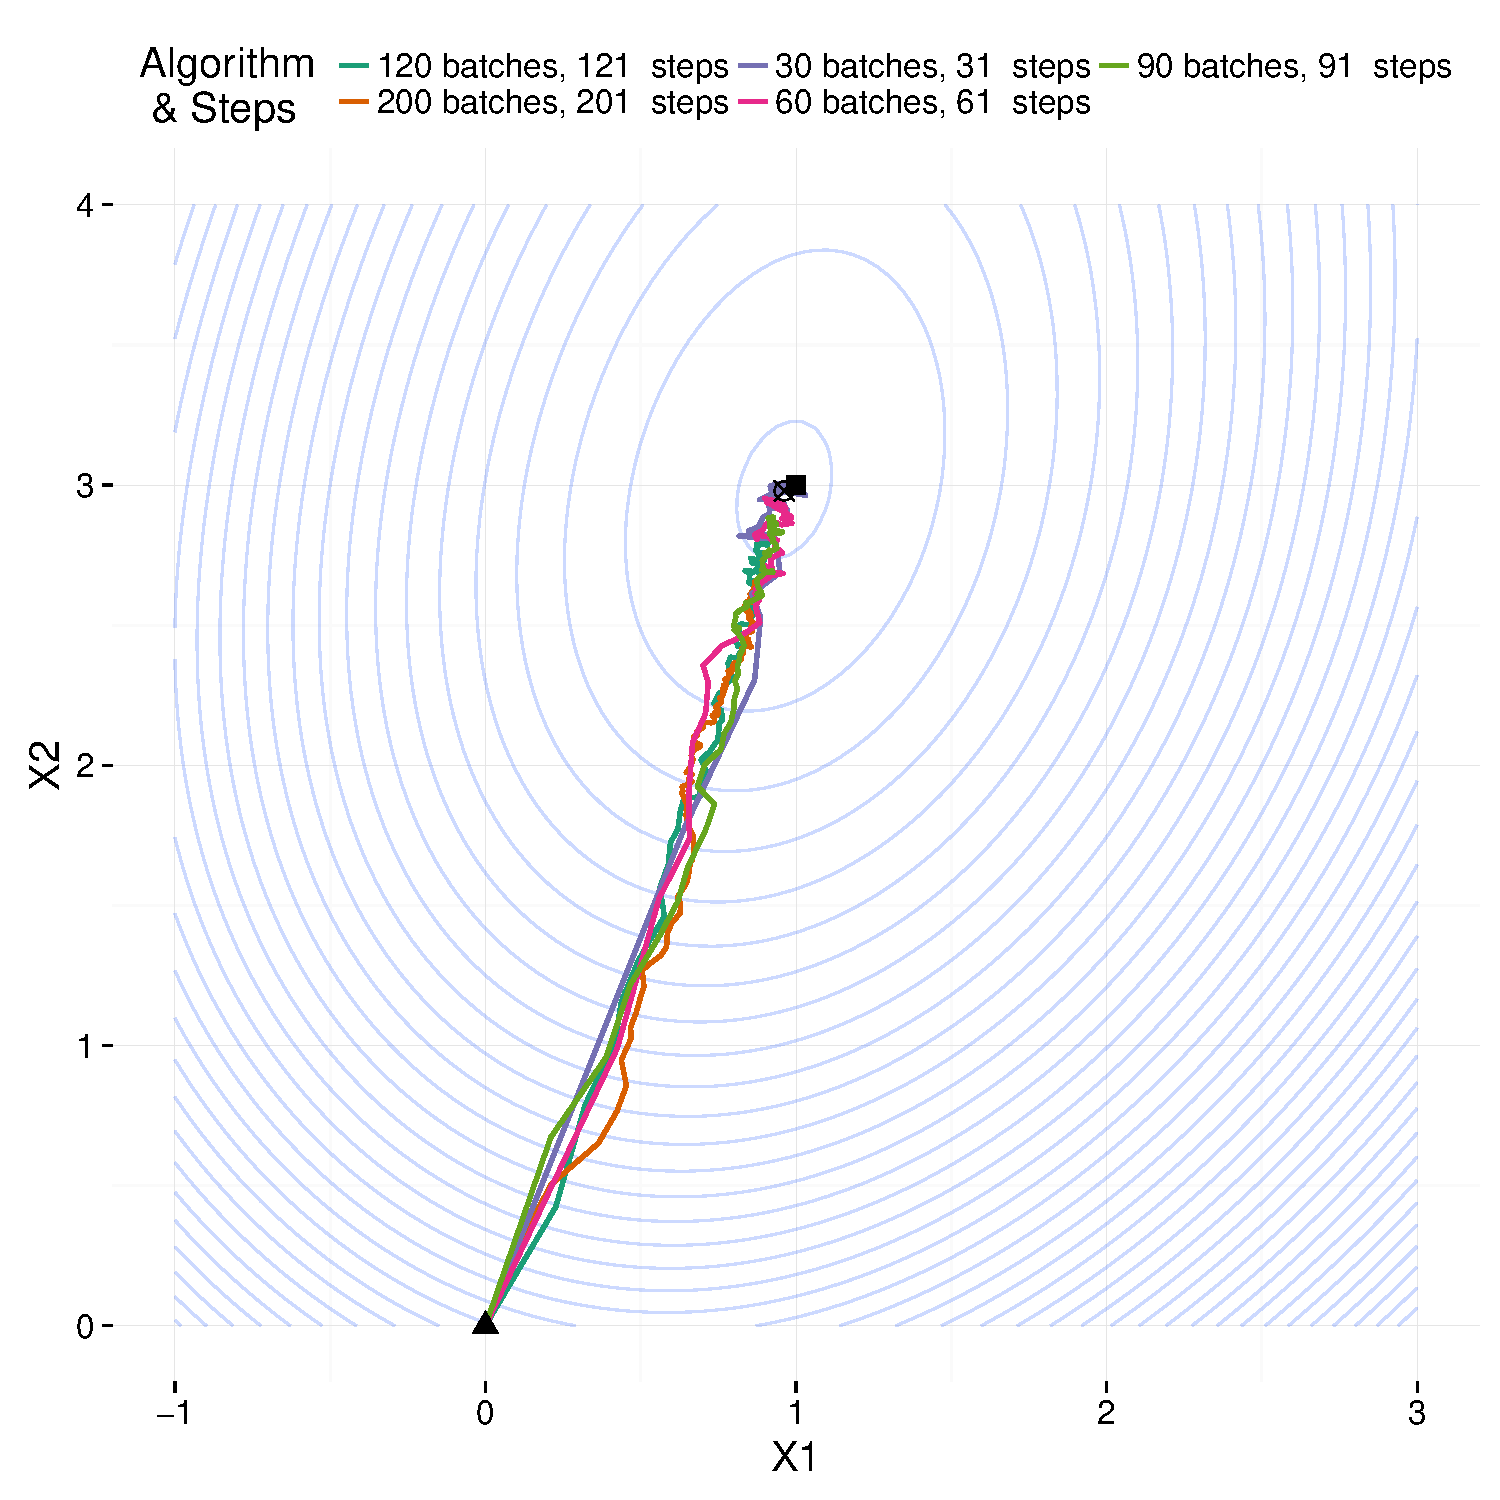
\includegraphics[width=\textwidth, height=310pt]{Obrazki/b_0_0_iter_1_e-6_50sqrt.pdf}
      \caption{$\beta_0=(0,0)$, liczba epok 1, warunek stopu: $\varepsilon=10^{-6}$, długości kroków = $\frac{1}{50\sqrt{t}}$.}
   \end{subfigure}     
   \begin{subfigure}[h!]{0.9\textwidth}
      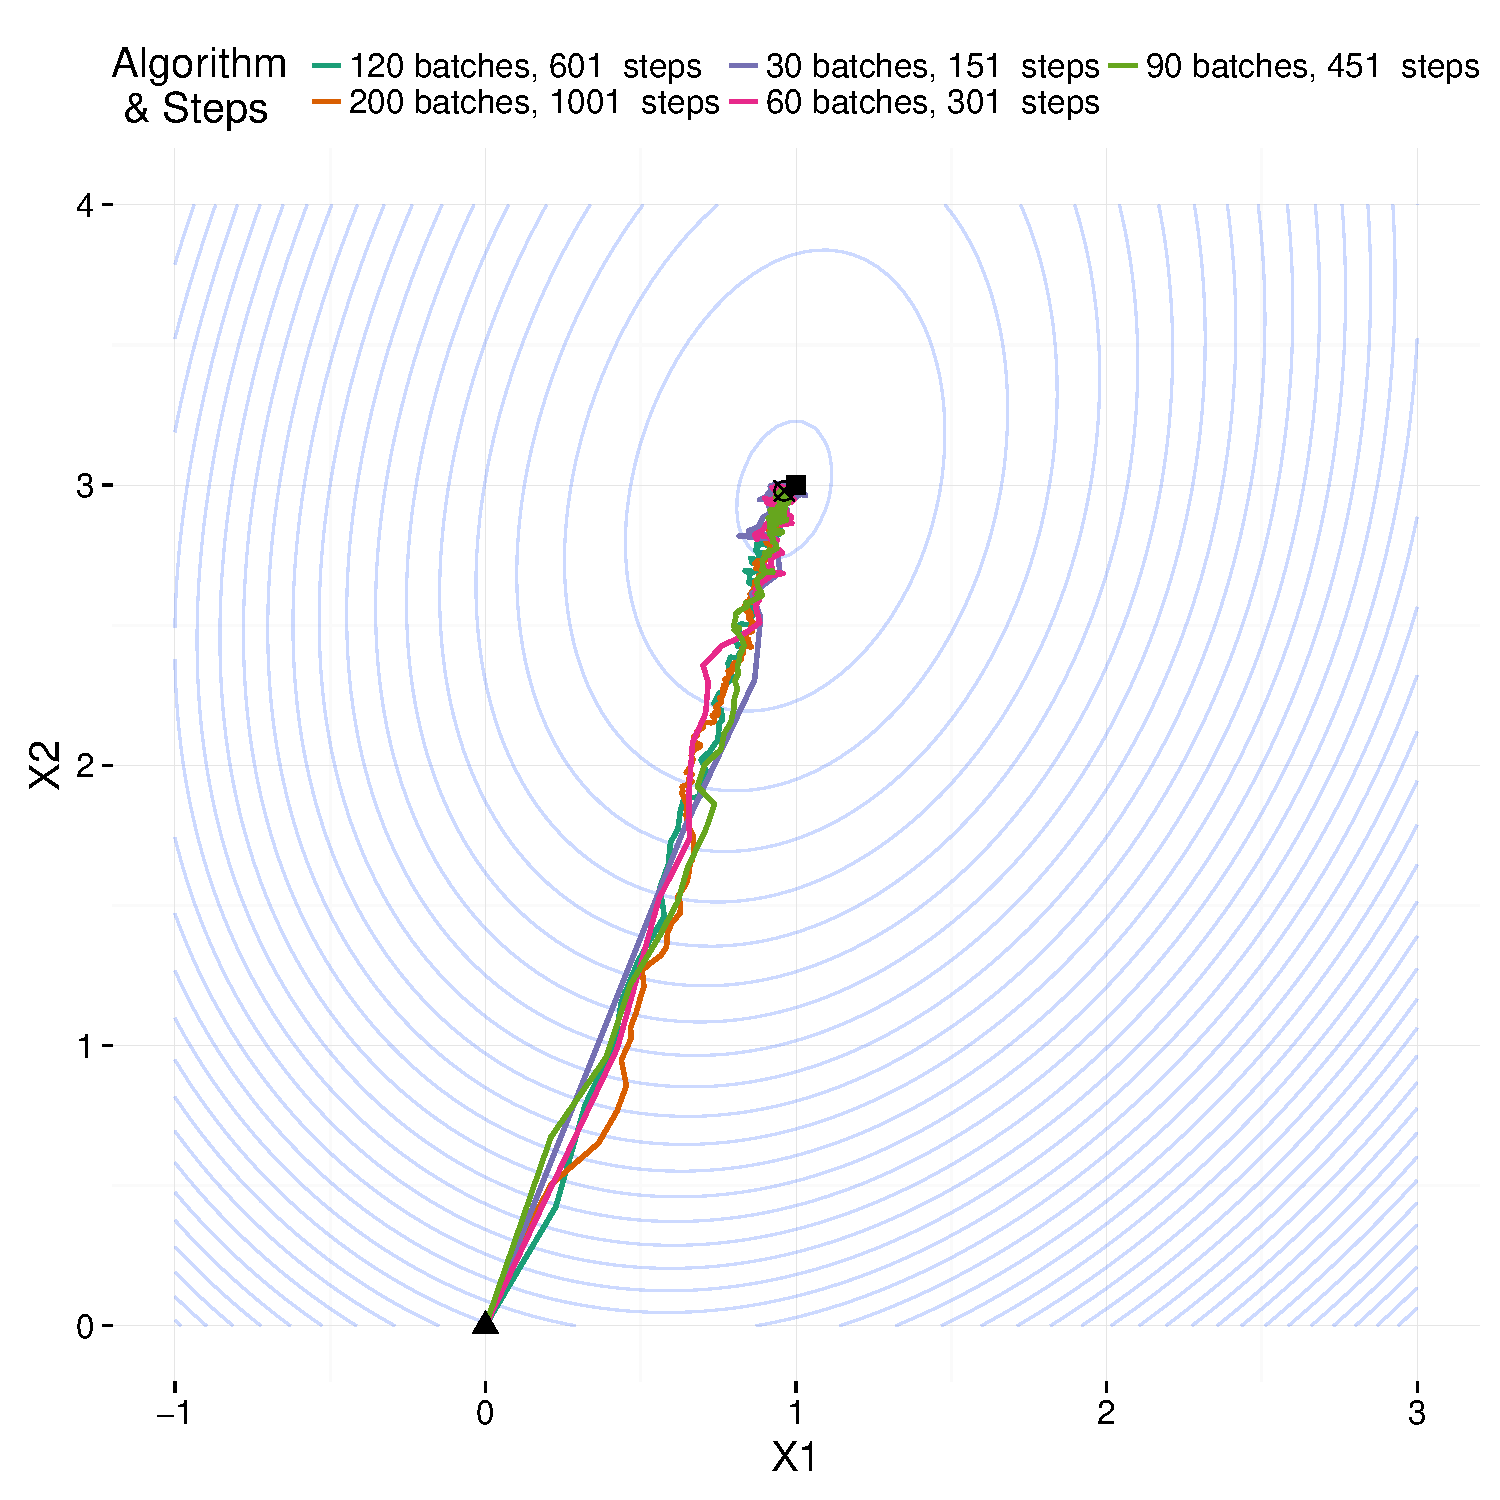
\includegraphics[width=\textwidth, height=310pt]{Obrazki/b_0_0_iter_5_e-6_50sqrt.pdf}
            \caption{$\beta_0=(0,0)$, liczba epok 5, warunek stopu: $\varepsilon=10^{-6}$, długości kroków = $\frac{1}{50\sqrt{t}}$.}
   \end{subfigure}  
      \end{center}
  %\vspace{-10pt}
  \caption[Porównanie trajektorii estymacji w modelu Coxa, wykorzystującym metodę stochastycznego spadku gradientu, przy różnych podziałach zbioru początkowego na podzbiory.]{\label{rysCox}Porównanie trajektorii estymacji w modelu Coxa, wykorzystującym metodę stochastycznego spadku gradientu, w zależności od różnych podziałów zbioru początkowego na podzbiory. Elipsami przedstawiono warstwice częściowej funkcji log-wiarogodności wyliczone na bazie wszystkich obserwacji. Trójkątem zaznaczono punkt startowy algorytmu, kwadratem teoretyczne maksimum, zaś gwiazdką współczynniki uzyskane za pomocą funkcji \texttt{coxph()}.}
\end{figure}



\begin{figure}[hbt!]
  %\vspace{-10pt}
  \begin{center}
   \begin{subfigure}[h!]{0.9\textwidth}
      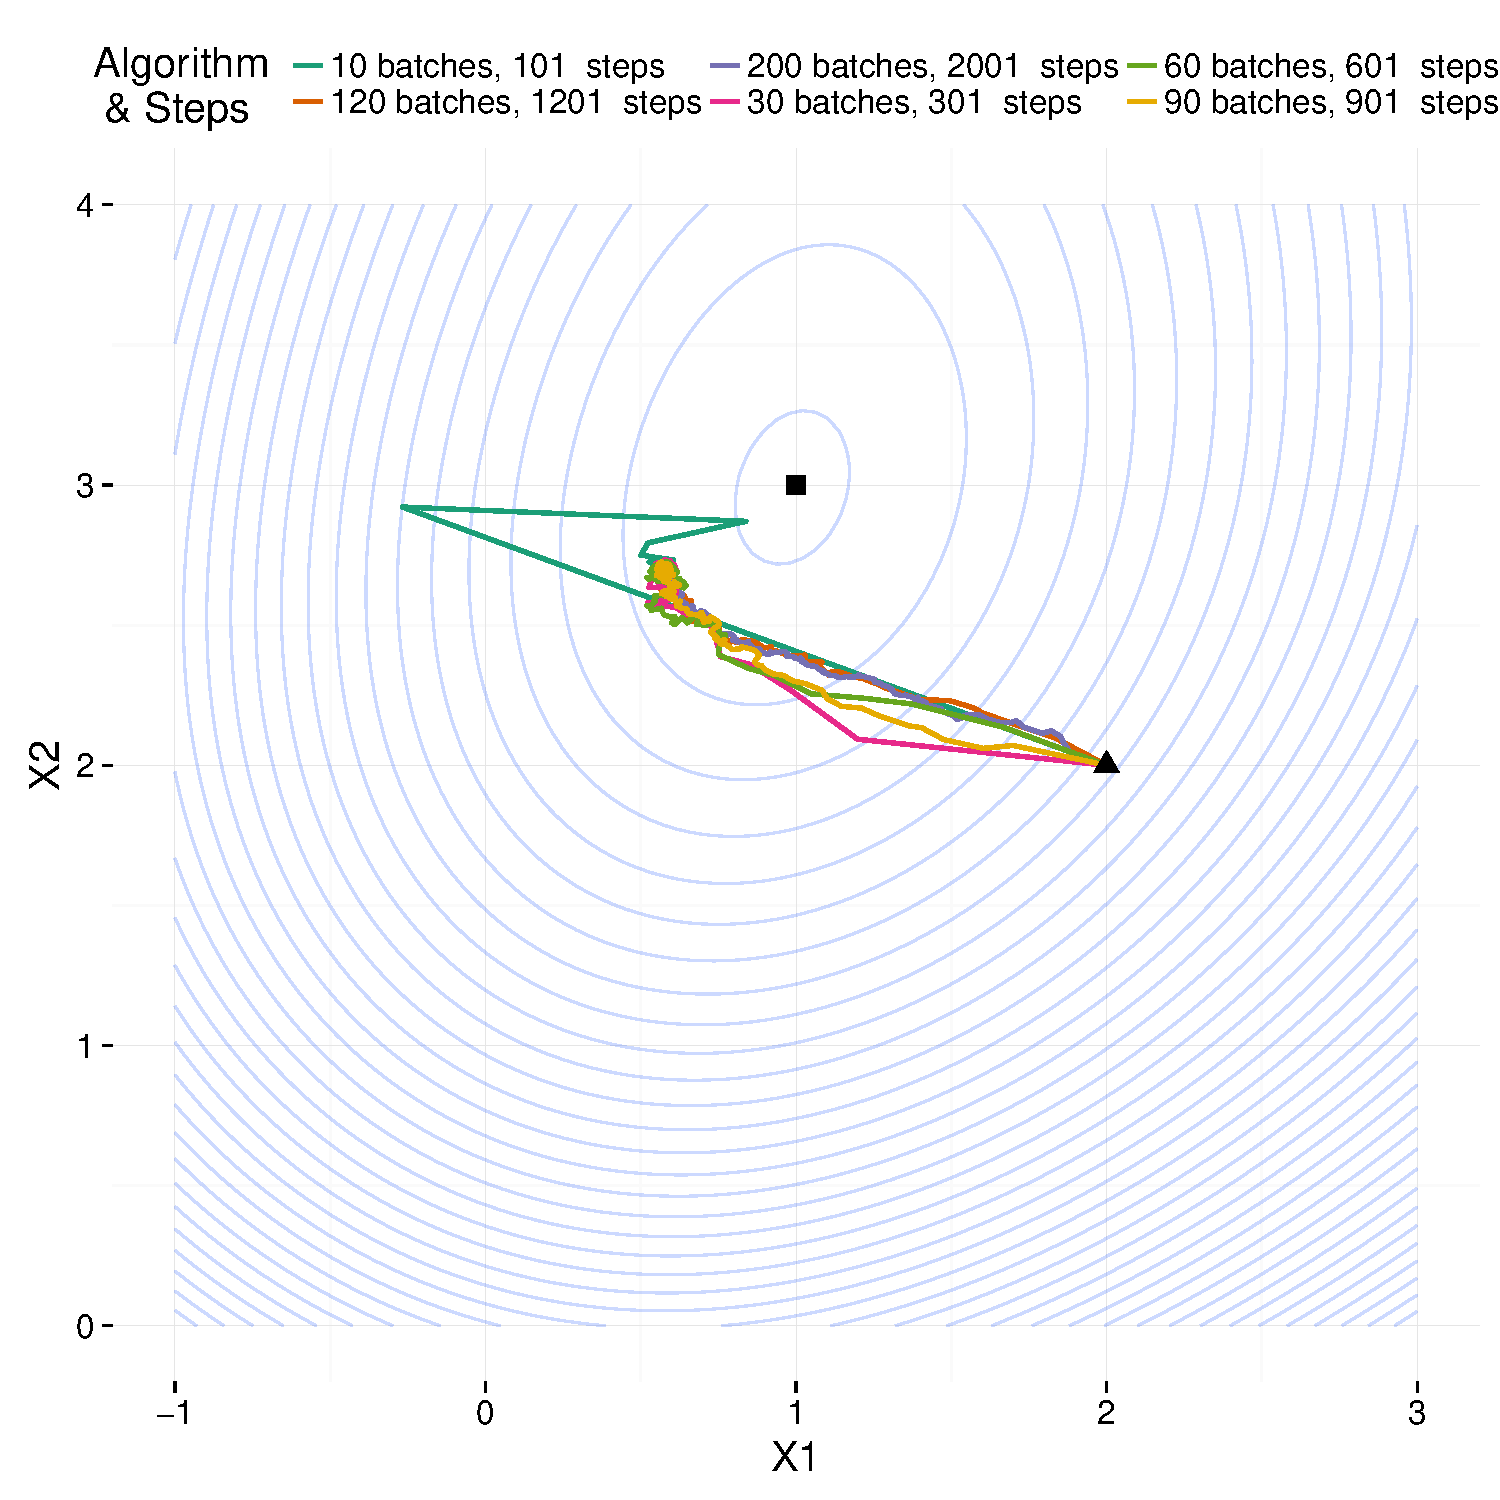
\includegraphics[width=\textwidth, height=310pt]{Obrazki/b_2_2_iter_10_e-6_50sqrt.pdf}
      \caption{$\beta_0=(2,2)$, liczba epok 10, warunek stopu: $\varepsilon=10^{-6}$, długości kroków = $\frac{1}{50\sqrt{t}}$.}
   \end{subfigure}     
   \begin{subfigure}[h!]{0.9\textwidth}
      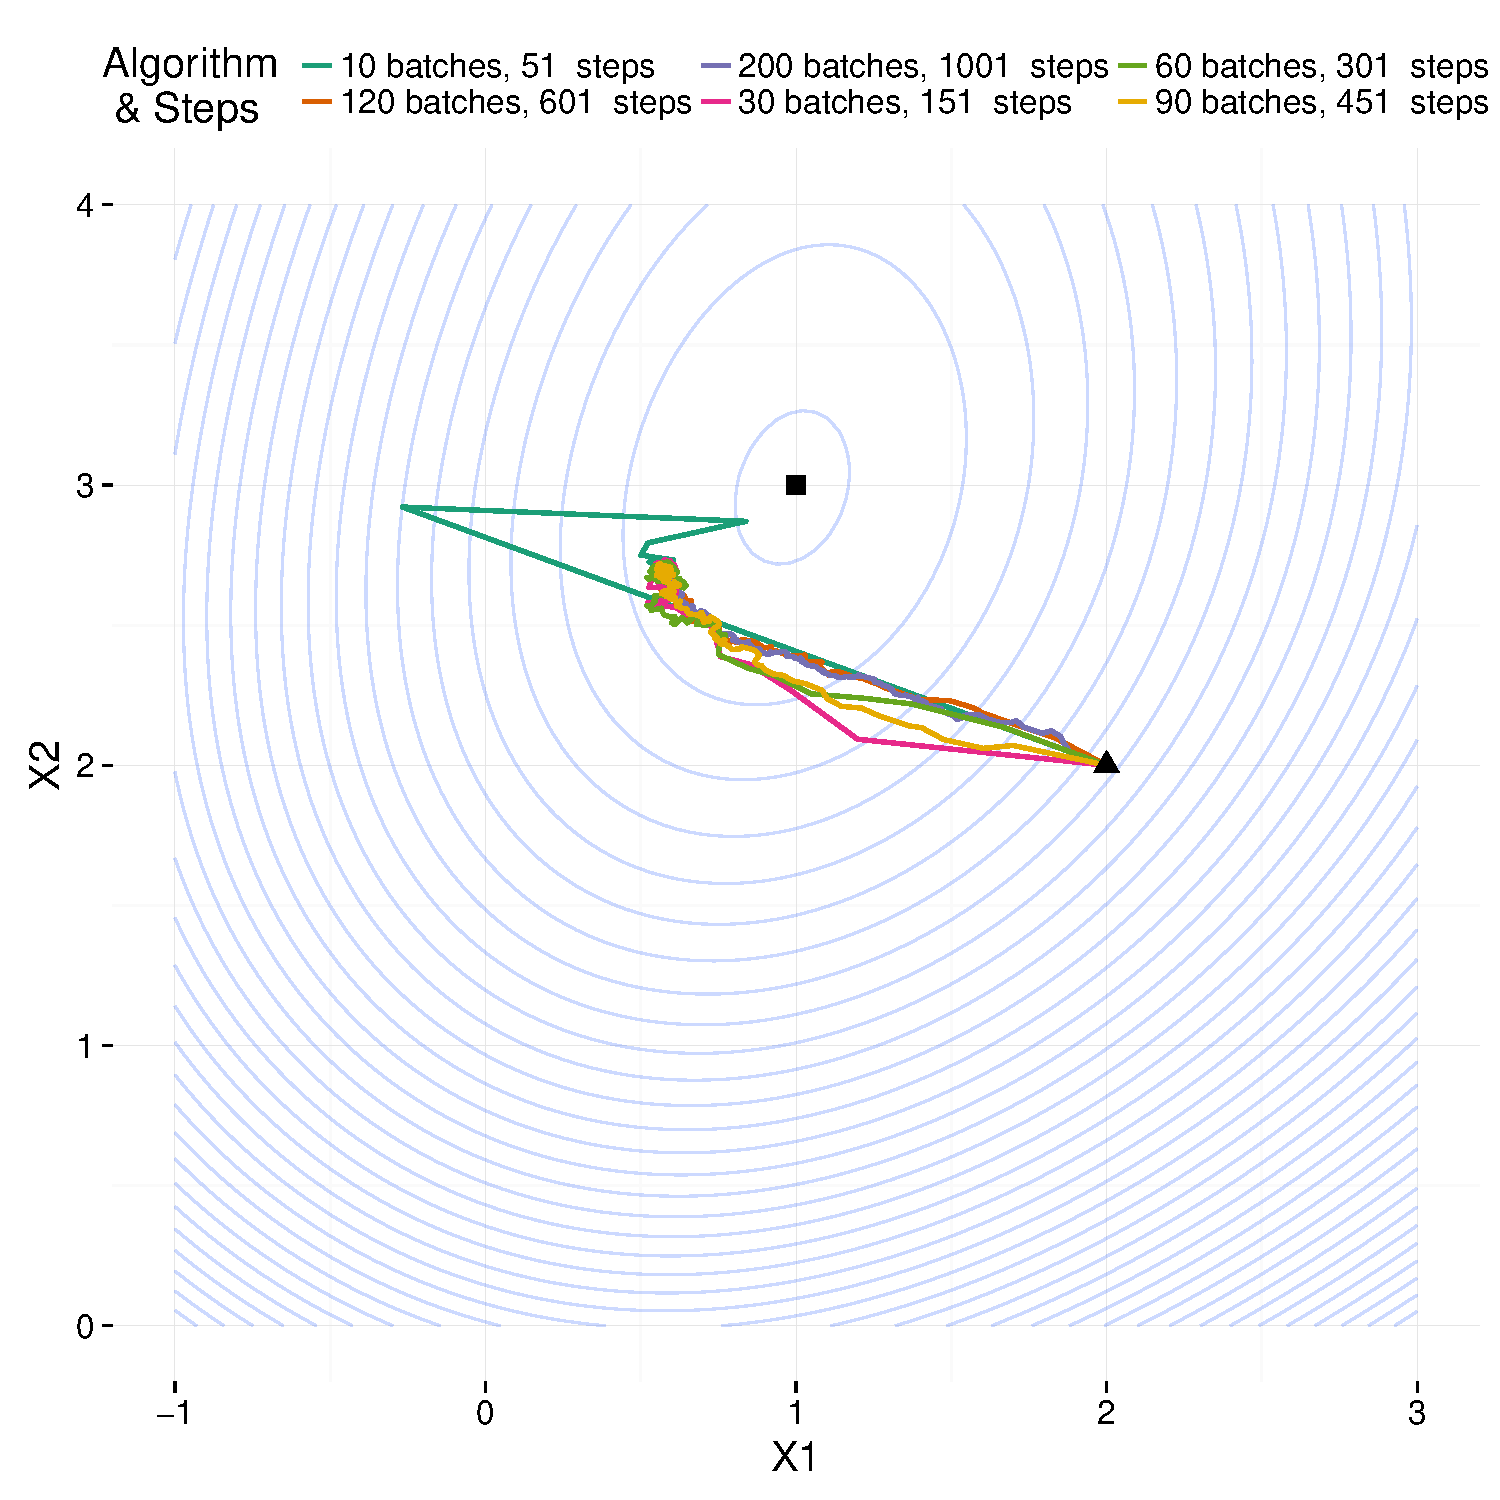
\includegraphics[width=\textwidth, height=310pt]{Obrazki/b_2_2_iter_5_e-5_50sqrt.pdf}
            \caption{$\beta_0=(2,2)$, liczba epok 5, warunek stopu: $\varepsilon=10^{-5}$, długości kroków = $\frac{1}{50\sqrt{t}}$.}
   \end{subfigure}  
      \end{center}
  %\vspace{-10pt}
  \caption[Porównanie estymacji w modelu Coxa metodą stochastycznego spadku gradientu dla różnych podziałów zbioru początkowego na podzbiory.]{\label{rysCox2}Porównanie trajektorii estymacji w modelu Coxa, wykorzystującym metodę stochastycznego spadku gradientu, w zależności od różnych podziałów zbioru początkowego na podzbiory. Elipsami przedstawiono warstwice częściowej funkcji log-wiarogodności wyliczone na bazie wszystkich obserwacji. Trójkątem zaznaczono punkt startowy algorytmu, kwadratem teoretyczne maksimum, zaś gwiazdką współczynniki uzyskane za pomocą funkcji \texttt{coxph()}.}
\end{figure}
	
	
	
	
\begin{figure}[hbt!]
  %\vspace{-10pt}
  \begin{center}
   \begin{subfigure}[h!]{0.9\textwidth}
      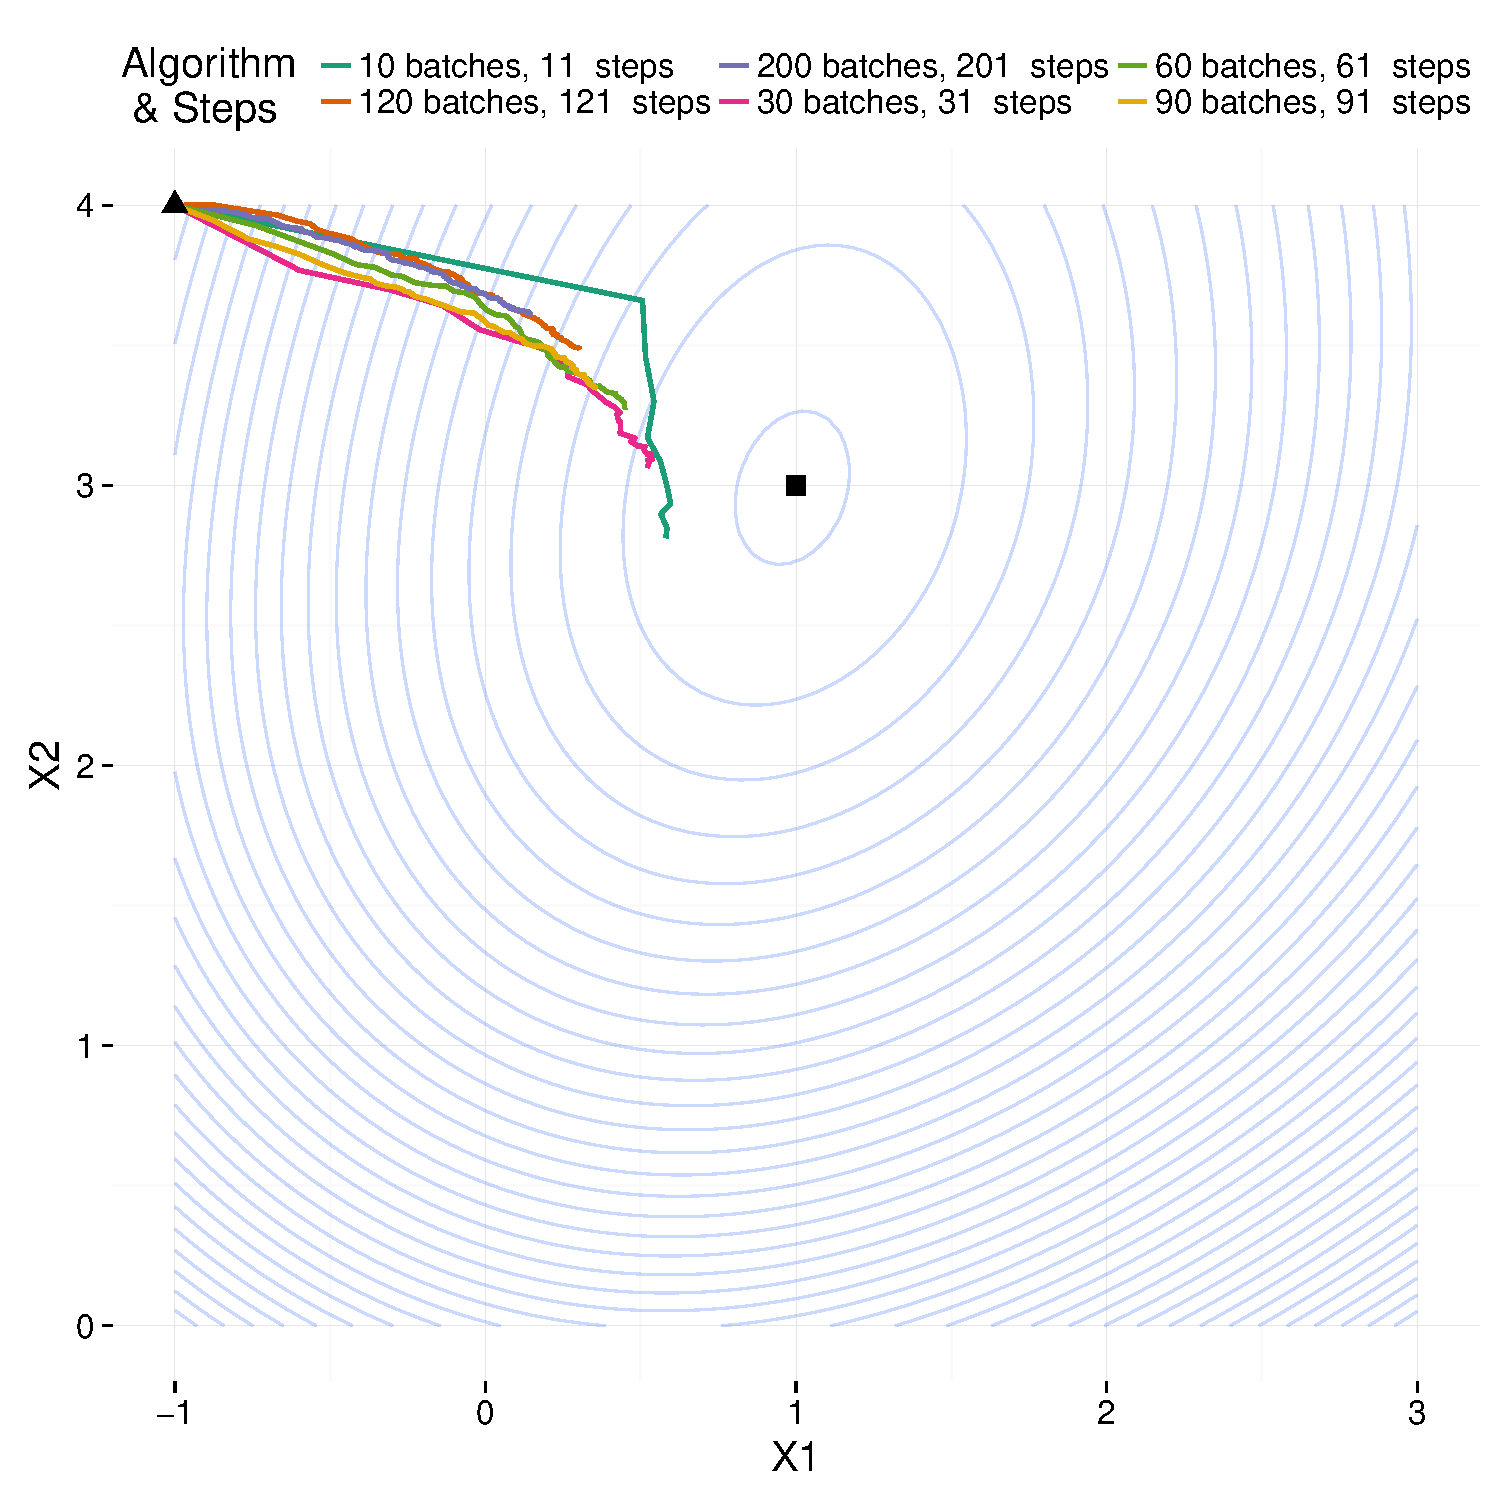
\includegraphics[width=\textwidth, height=310pt]{Obrazki/b_m1_4_iter_1_e-6_100sqrt.pdf}
      \caption{$\beta_0=(-1,4)$, liczba epok 1, warunek stopu: $\varepsilon=10^{-6}$, długości kroków = $\frac{1}{100\sqrt{t}}$.}
   \end{subfigure}     
   \begin{subfigure}[h!]{0.9\textwidth}
      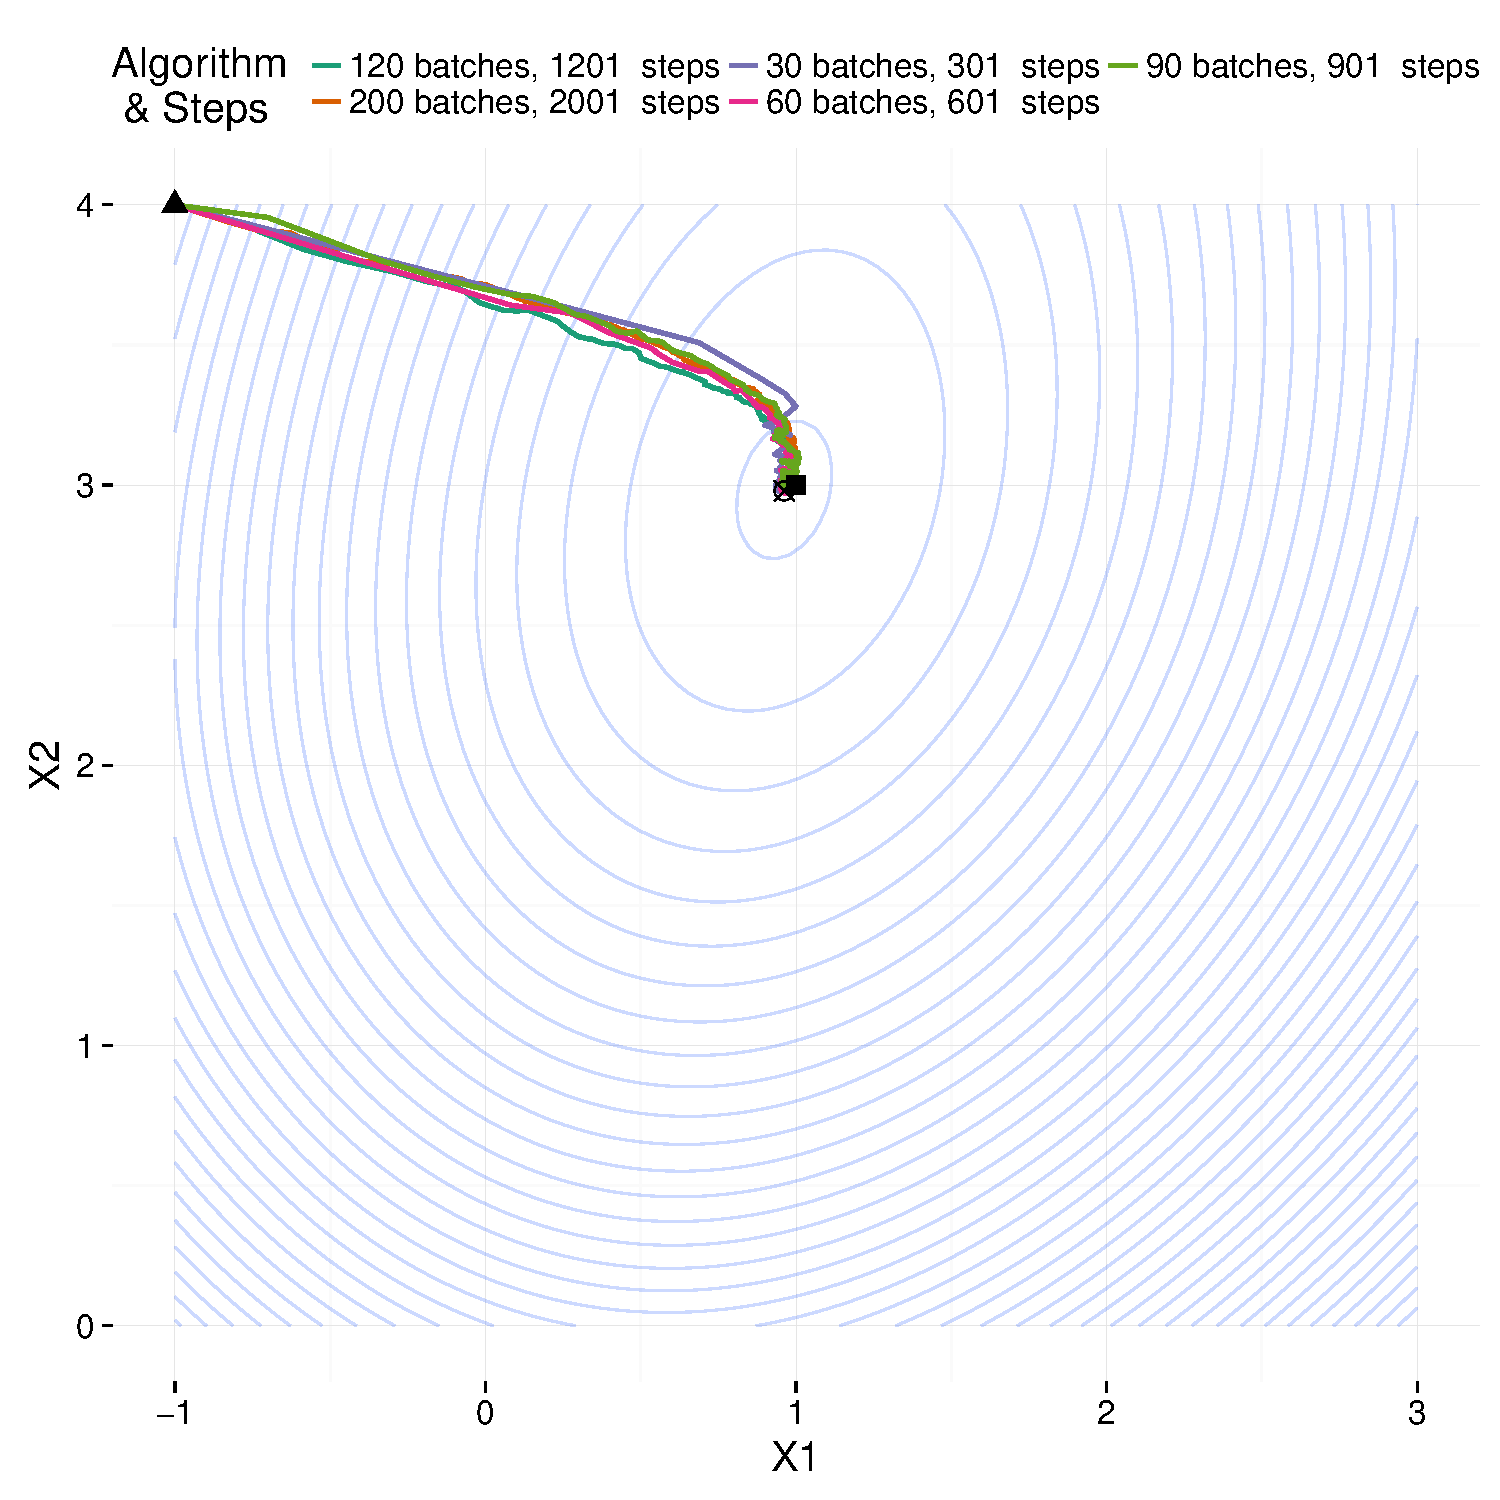
\includegraphics[width=\textwidth, height=310pt]{Obrazki/b_m1_4_iter_10_e-5_100sqrt.pdf}
            \caption{$\beta_0=(-1,4)$, liczba epok 10, warunek stopu: $\varepsilon=10^{-5}$, długości kroków = $\frac{1}{100\sqrt{t}}$.}
   \end{subfigure}  
      \end{center}
  %\vspace{-10pt}
  \caption[Porównanie estymacji w modelu Coxa metodą stochastycznego spadku gradientu dla różnych podziałów zbioru początkowego na podzbiory.]{\label{rysCox3}Porównanie trajektorii estymacji w modelu Coxa, wykorzystującym metodę stochastycznego spadku gradientu, w zależności od różnych podziałów zbioru początkowego na podzbiory. Elipsami przedstawiono warstwice częściowej funkcji log-wiarogodności wyliczone na bazie wszystkich obserwacji. Trójkątem zaznaczono punkt startowy algorytmu, kwadratem teoretyczne maksimum, zaś gwiazdką współczynniki uzyskane za pomocą funkcji \texttt{coxph()}.}
\end{figure}



\begin{figure}[hbt!]
  %\vspace{-10pt}
  \begin{center}
   \begin{subfigure}[h!]{0.9\textwidth}
      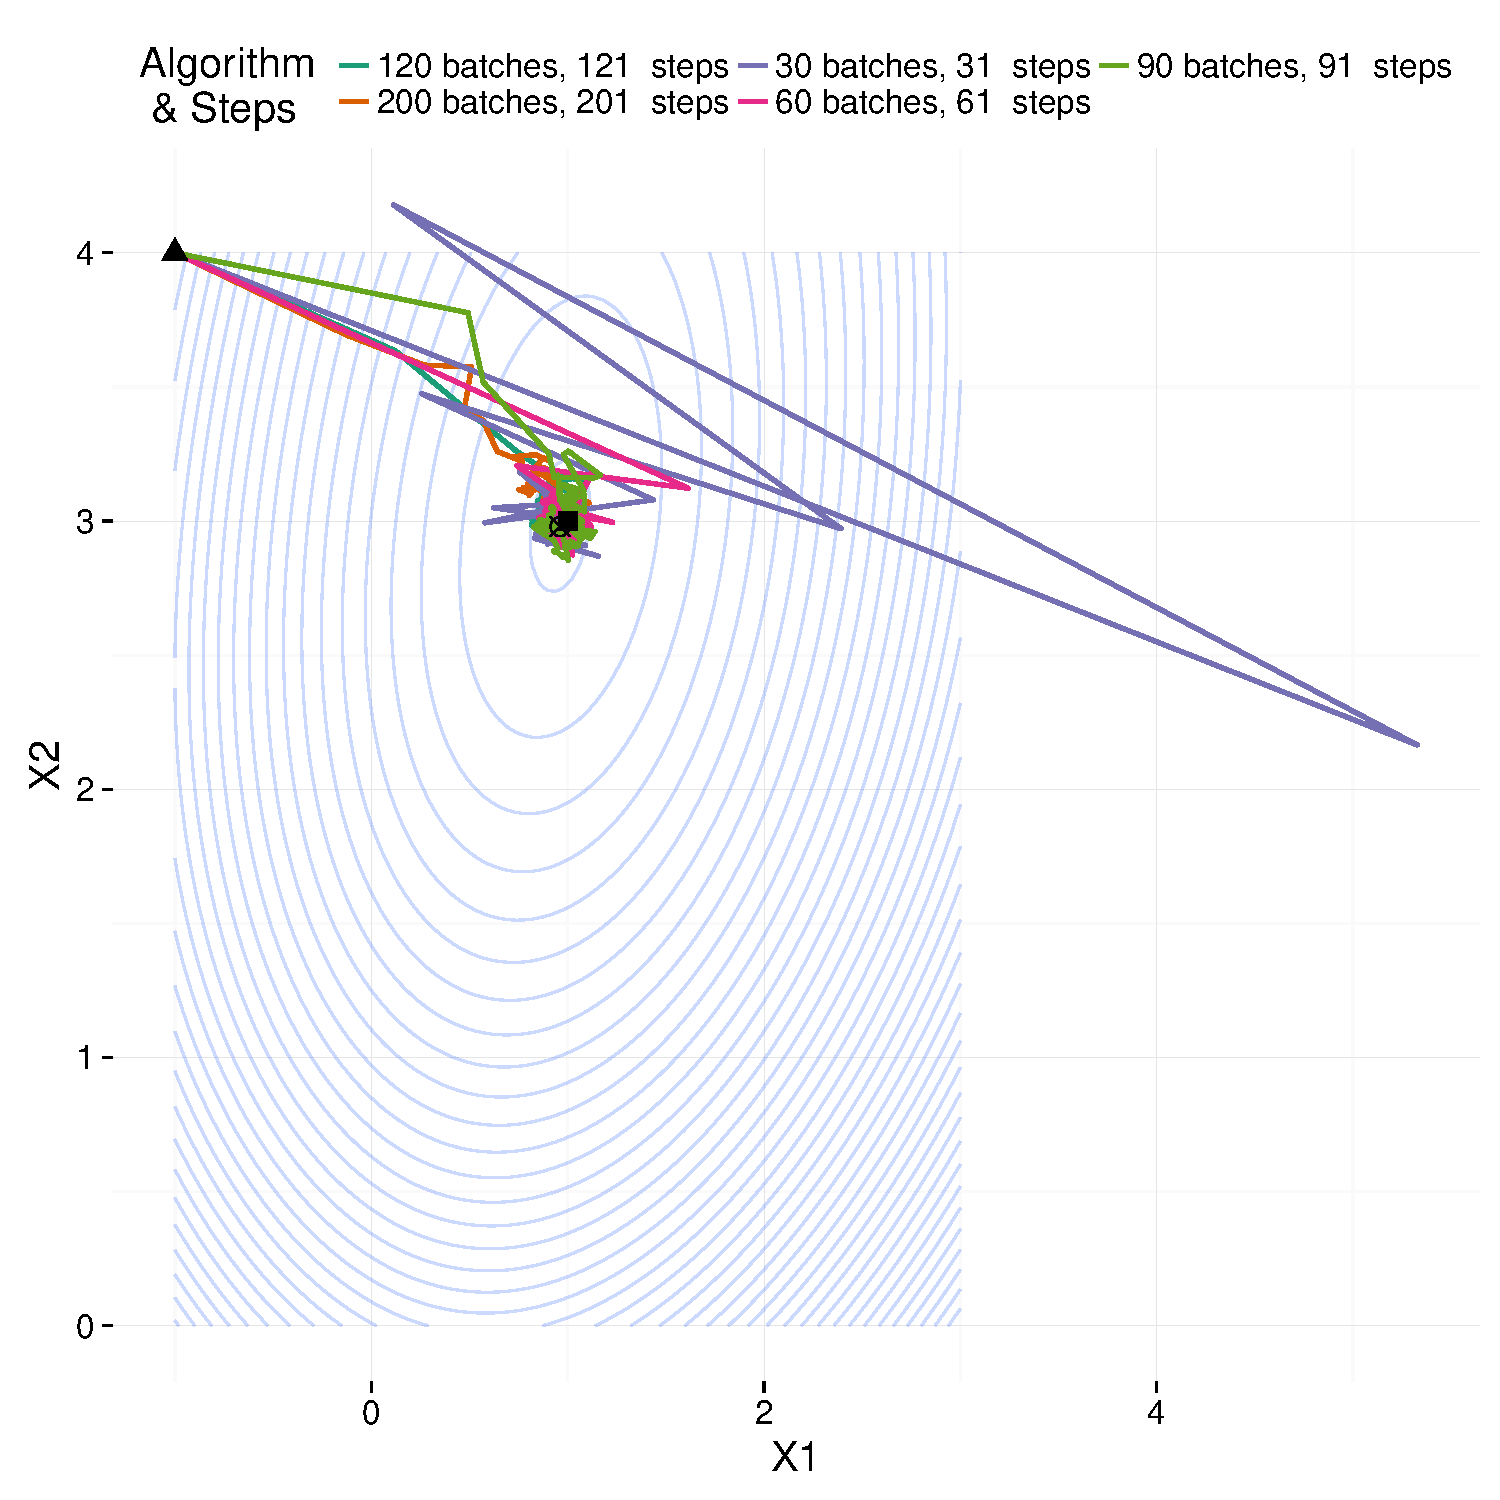
\includegraphics[width=\textwidth, height=310pt]{Obrazki/b_m1_4_iter_1_e-6_20sqrt.pdf}
      \caption{$\beta_0=(-1,4)$, liczba epok 1, warunek stopu: $\varepsilon=10^{-6}$, długości kroków = $\frac{1}{20\sqrt{t}}$.}
   \end{subfigure}     
   \begin{subfigure}[h!]{0.9\textwidth}
      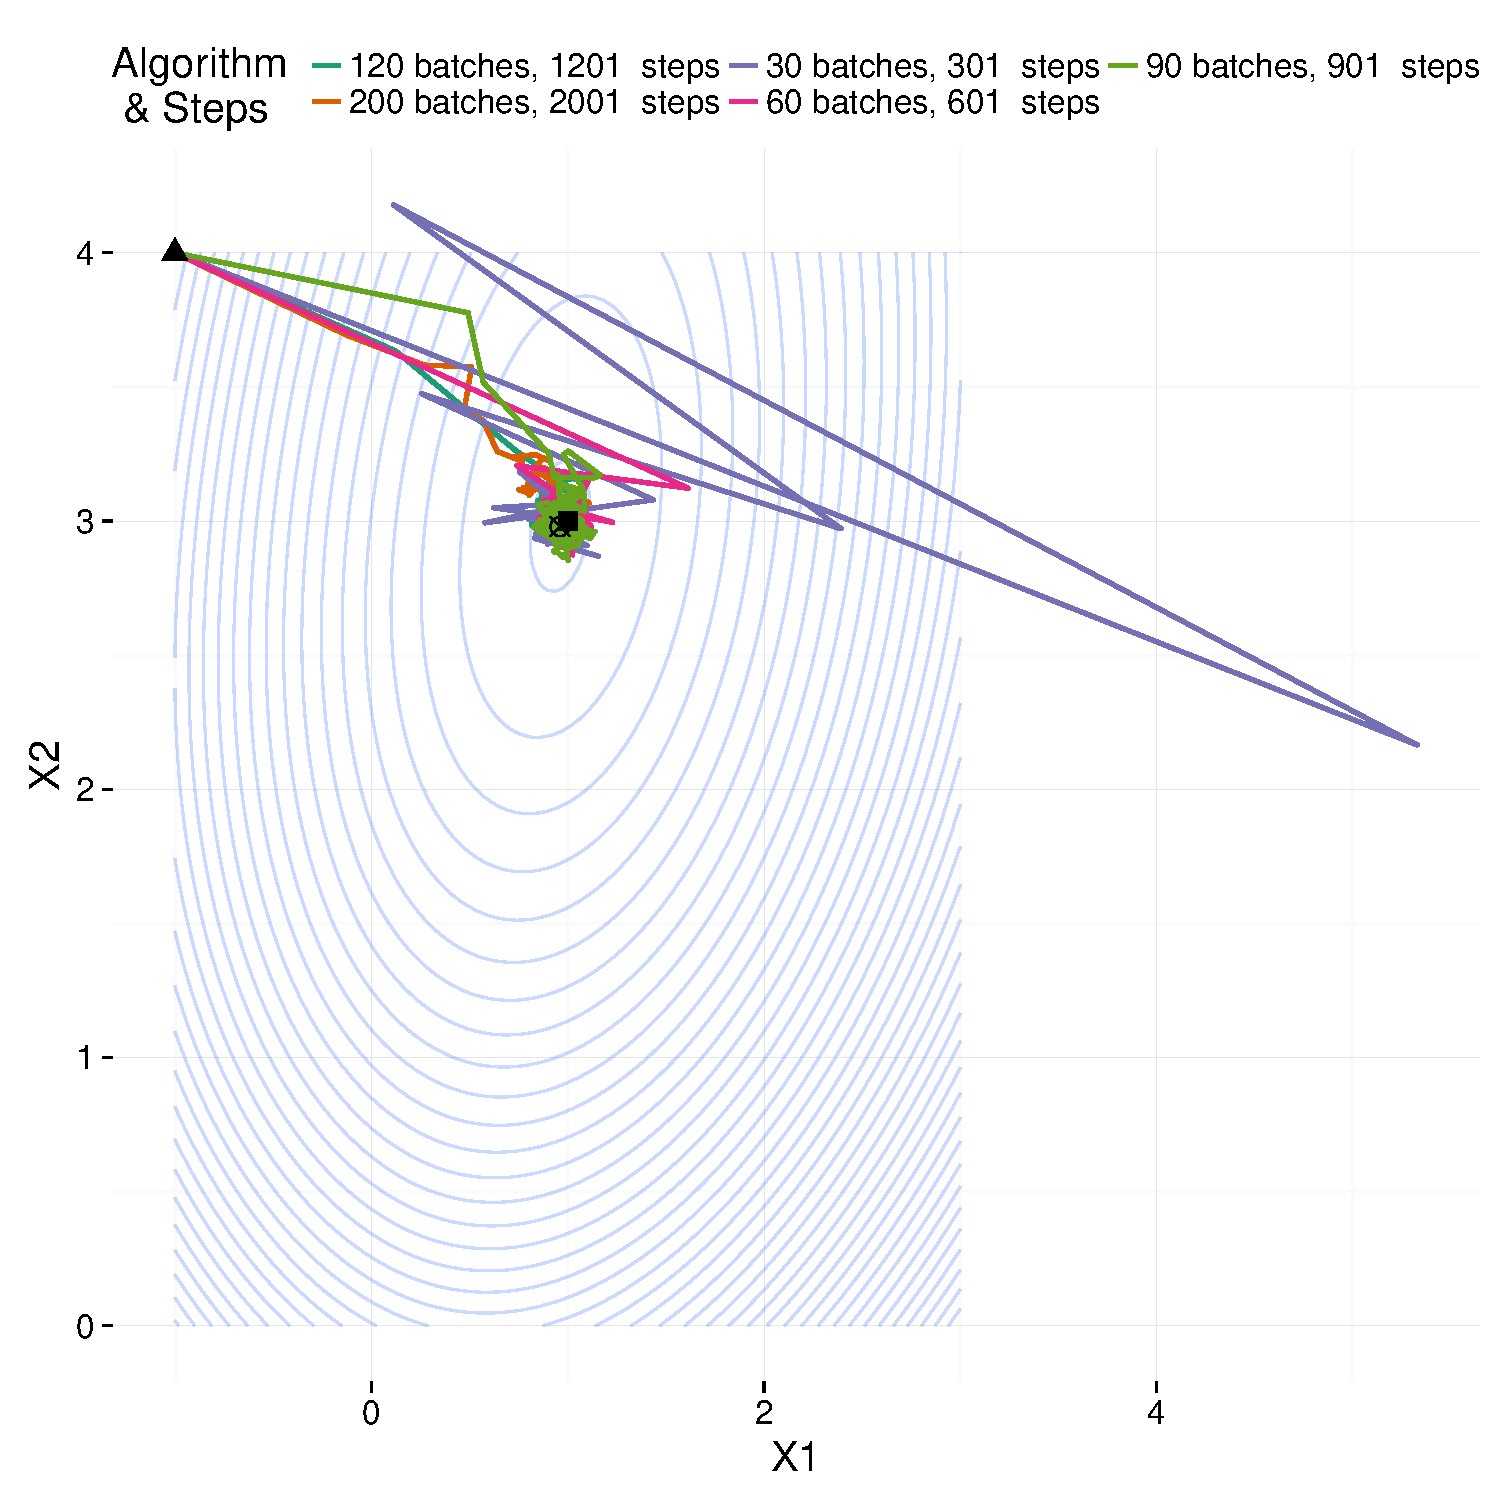
\includegraphics[width=\textwidth, height=310pt]{Obrazki/b_m1_4_iter_10_e-5_20sqrt.pdf}
            \caption{$\beta_0=(-1,4)$, liczba epok 10, warunek stopu: $\varepsilon=10^{-5}$, długości kroków = $\frac{1}{20\sqrt{t}}$.}
   \end{subfigure}  
      \end{center}
  %\vspace{-10pt}
  \caption[Porównanie estymacji w modelu Coxa metodą stochastycznego spadku gradientu dla różnych podziałów zbioru początkowego na podzbiory.]{\label{rysCox4}Porównanie trajektorii estymacji w modelu Coxa, wykorzystującym metodę stochastycznego spadku gradientu, w zależności od różnych podziałów zbioru początkowego na podzbiory. Elipsami przedstawiono warstwice częściowej funkcji log-wiarogodności wyliczone na bazie wszystkich obserwacji. Trójkątem zaznaczono punkt startowy algorytmu, kwadratem teoretyczne maksimum, zaś gwiazdką współczynniki uzyskane za pomocą funkcji \texttt{coxph()}.}
\end{figure}